\subsection{Comprehending Module Dependencies in Real Software}
\label{sec:apply}

We now give some usage scenarios which demonstrate how our visualizations
make it easier to understand the web of dependencies of software in Windows.
The dependencies shown are from programs runs in each
example and show how programs and binaries used in those runs
relate to one another.
The figures in this chapter are all scalable and thus can be magnified
in the PDF to see more detail and we encourage readers to do so.
In this section,
the files in some nodes in the graphs are abbreviated to $(\ldots)$ to make
it easier to fit the graphs in the thesis.
All the DLL dependency graphs remove dependencies due to
DLL initialization.\footnote{
One could choose also to see DLL initialization dependencies, as removal
would not make sense for DLLs which do significant work in the initialization.
}

\subsubsection{System Boot}
\label{sec:apply:boot}

\begin{figure*}[htbp]
\centering
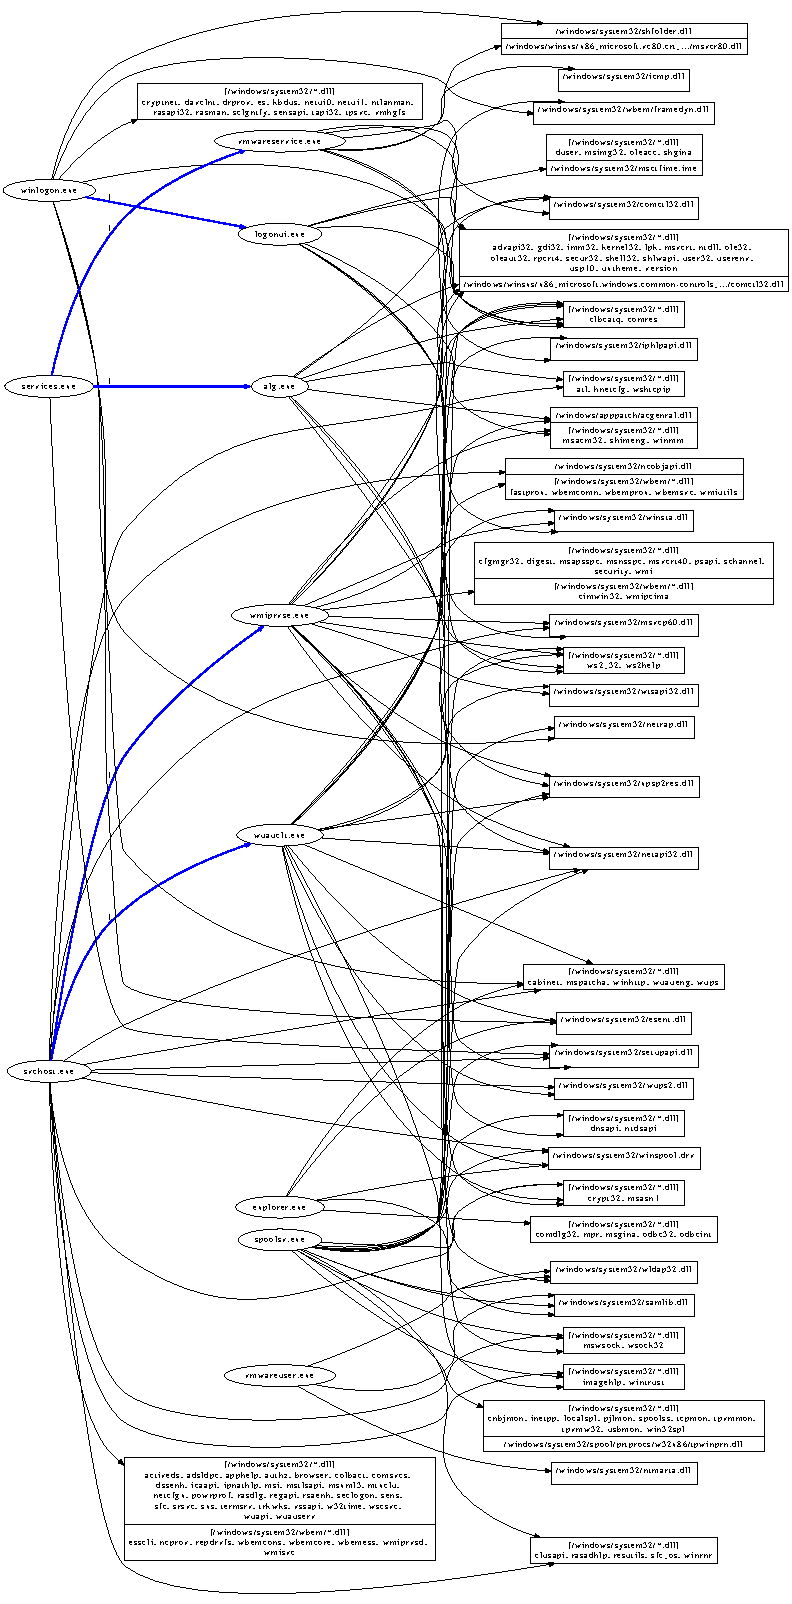
\includegraphics[keepaspectratio,width=0.95\textwidth,height=0.95\textheight]{depvis/boot-gdll.pdf}
\caption{EXE dependency graph of the whole system}
\label{fig:boot}
\end{figure*}

Figure~\ref{fig:boot} shows the EXE dependency graph for a boot to shutdown cycle
for a fresh Windows XP install.
The machine was booted and automatically logged in,
then logged off, and shutdown. One might expect that the processes
form a process tree but that is not the case because some of the processes (e.g
svchost, winlogon, services) start before our monitoring tool
(WinResMon) does. Looking at the big picture of the startup and shutdown
process, it can be seen that some DLLs are shared by many programs (e.g
{\tt kernel32}, {\tt gdi32} and this is expected since system calls would use
{\tt kernel32} while GUI programs would use {\tt gdi32}).
On the other hand, some DLLs are used exclusively by one program (e.g.
{\tt odbc32} is used only by {\tt explorer}).
This is somewhat surprising leading to the question why {\tt odbc32},
the database query interface, is used by {\tt explorer}.

\subsubsection{Comparing Web Browsers}

\begin{figure}[bthp]
\centering
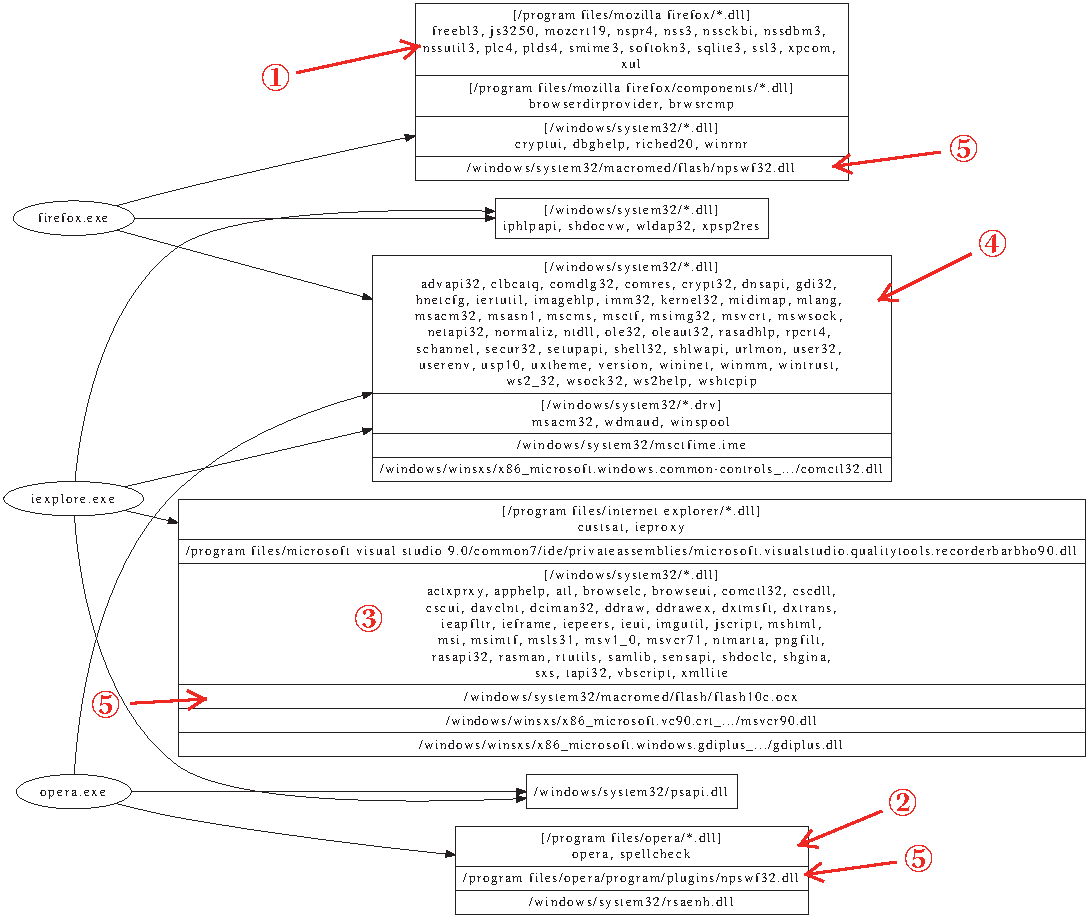
\includegraphics[width=1.0\textwidth]{depvis/browsers-group-annot.pdf}
\caption{EXE dependency graph of three browsers: IE, Firefox, Opera}
\label{fig:browsers}
\end{figure}

\begin{sidewaysfigure}
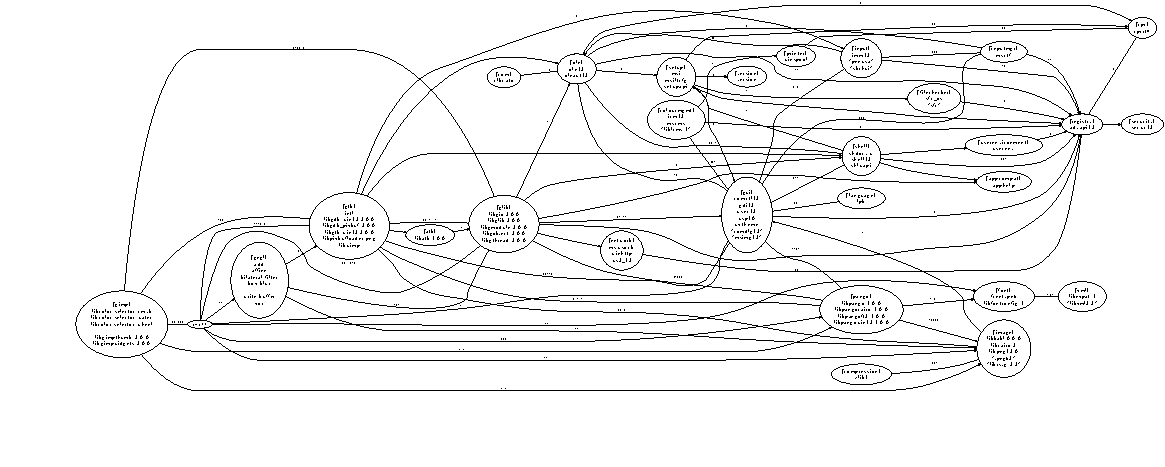
\includegraphics[width=1.0\textwidth]{depvis/gimp-function-removed.pdf}
\caption{DLL dependency graph of Gimp grouped by functionality}
\label{fig:gimp-function}
\end{sidewaysfigure}

Figure~\ref{fig:browsers} shows the EXE dependency graph for three
brow\-sers: Internet Explorer, Firefox and Opera.
Each browser displayed a YouTube page to play a
video till completion. The scenario is intended to show the dependencies
of the binaries used by the three programs
with similar function but different source code base.
The visualization shows the commonalities and differences
between the software modules in the three browsers.
It also shows dependencies on other software which is not part of
the browser code base and
which comes in through the use of browser extensions or plugins,
e.g. Adobe Flash.

This example shows the compressed EXE dependency gra\-ph
with grouping.
We see that grouping makes the graph easier to visualize.
Firstly, the grouped version is much smaller in size.
Secondly, it is easier to identify which binaries are shared by the same programs.
We have highlighted particular nodes in the graph with
labels, the numbered red arrows, discussed below:
\begin{itemize}


\item Labels 1, 2 and 3 show the DLLs used exclusively by Firefox, Opera
and Internet Explorer respectively. Opera does not have many  of its own DLLs.
On the other hand, Firefox uses its own DLLs (in {\tt /program files/mozilla firefox}) for many features.
In the case of Internet Explorer, the ownership of the DLLs are less clear
since most of the DLLs used come from the {\tt system32} directory.
This may be due to the deeper integration of Internet Explorer with
Windows.

\item Label 4 shows the common binaries shared by all three browsers.
It is not surprising that a large number of binaries are shared.
This is because most of the major Win32 API calls
are implemented in those binaries, e.g.
\texttt{msacm32.drv} and \texttt{wdmaud.drv},
are the audio drivers that all browsers use to play the video.


\item Label 5 shows the different ways that each browser runs Flash.
In Internet Explorer,
Flash is installed as an ActiveX control (\texttt{flash10c.ocx}).
Firefox and Opera both use (\texttt{npswf32.dll}), the Flash plugin
for Netscape. We discover that the same DLL is duplicated in
different directories.

\end{itemize}

\subsubsection{Gimp}

\begin{sidewaysfigure}
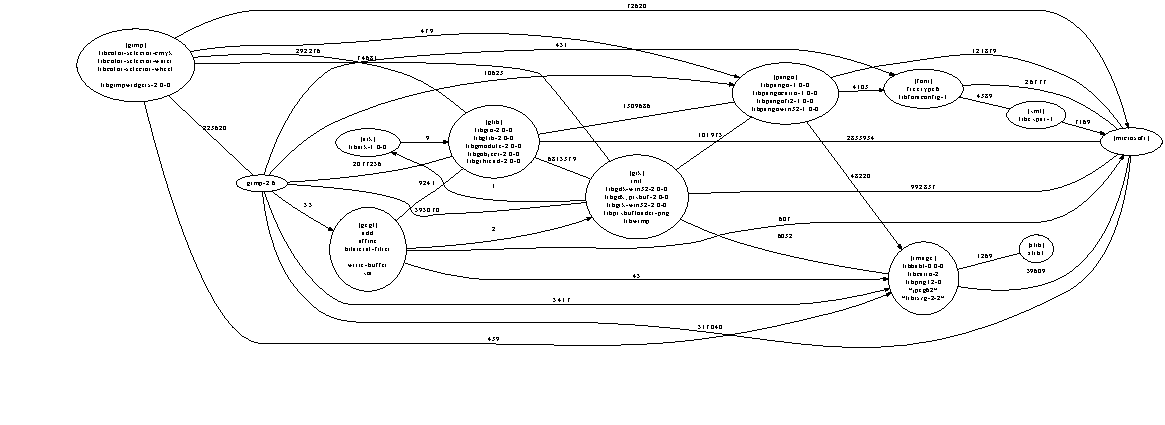
\includegraphics[width=1.0\textwidth]{depvis/gimp-vendor.pdf}
\caption{DLL dependency graph of Gimp grouped by software vendor}
\label{fig:gimp-vendor}
\end{sidewaysfigure}

GIMP is an open source image manipulation program. Like many open source
software, it uses libraries from various sources. In this experiment, we
executed GIMP without opening any files. We want to see how GIMP uses various
libraries and the interactions between them.

Figure~\ref{fig:gimp-function} shows GIMP grouped by functionality while
Figure~\ref{fig:gimp-vendor} shows
GIMP grouped by software vendor.
GIMP is large but quite modular. The bulk of
the DLLs used are from the GEGL, GTK and GLIB frameworks. It also uses the
Windows GUI APIs (e.g., gdi32, comctl32) extensively.

Figure~\ref{fig:gimp-function} is a larger graph than Figure~\ref{fig:gimp-vendor}
but is still understandable using the functional grouping,
e.g. {\tt gimp} uses the {\tt [gegl]}
image processing modules, which in turn uses the {\tt [gtk]} windowing
module.  The remaining DLLs are not used very much.

Figure~\ref{fig:gimp-vendor} is interesting because it shows that
many different software vendors/providers are used in GIMP.
Microsoft is also prominent but is
expected since GIMP is running on Windows and uses the Win32 API.
The presence of so many different software vendors could also make
troubleshooting difficult since it might be difficult to determine
which vendor is responsible if GIMP behaves in unexpected ways.
Figure~\ref{fig:gimp-vendor} also shows
one of the advantages of open source software, namely, reuse. The
binaries belonging to GIMP only turn out to be quite small and
GIMP prefers to rely on
existing frameworks like {\tt gtk} (GUI) and GEGL (image processing).

\subsubsection{Firefox: Plug-ins and a Surprise}

\begin{figure}
\centering
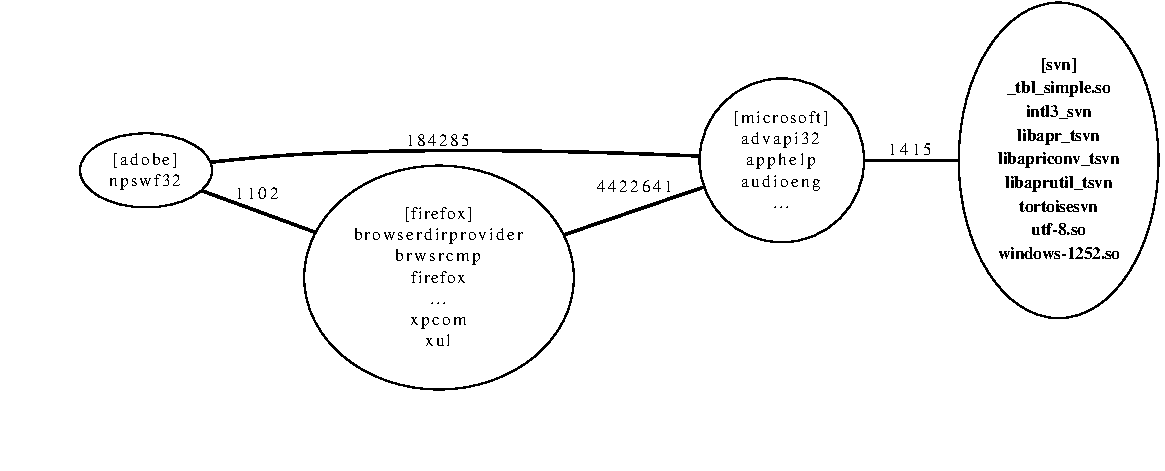
\includegraphics[width=1.0\columnwidth]{depvis/firefox-vendor.pdf}
\caption{DLL dependency graph of Firefox grouped by software vendor}
\label{fig:firefox}
\end{figure}

Firefox allows extensions through its own plug-in architecture.
Figure~\ref{fig:firefox} shows the DLL dependency graph
of Firefox as grouped by vendor. We find a node for Adobe.
This is because {\tt npswf32} is the Flash plugin for firefox.

We discover a surprising node -
the {\tt svn} vendor group (shown in bold font) which is to do with
the TortoiseSvn interface to SubVersion (the version control system).
TortoiseSvn is unrelated to either Firefox plugins or addons.
Thus, one might find its presence strange, when Firefox is being executed.
The explanation lies in the way the Tortoise shell extension
behaves in Windows. TortoiseSvn injects its DLLs into the
{\tt Explorer} shell process when Windows starts.
When explorer runs a process, the TortoiseSvn
DLLs are also loaded into the new process.
The fact that there is interaction with a module which is not part of
the Firefox can mean that a bug in that module can also affect Firefox.
This can be concern for software developers.

\subsubsection{Adobe Flash in Internet Explorer}
\label{sec:flash}

\begin{figure}
\centering
\noindent\makebox[\textwidth]{
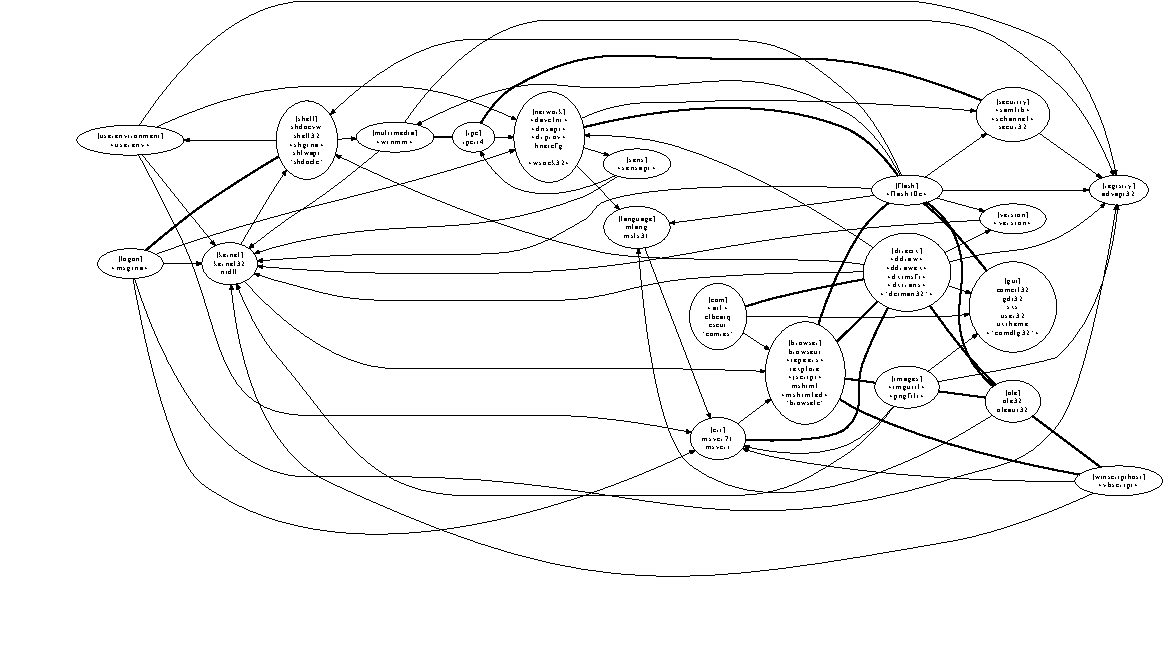
\includegraphics[width=1.2\textwidth]{depvis/ie-yt-diff.pdf}
}
\caption{Diff of DLL dependency graph of Internet Explorer with Flash and without}
\label{fig:ie-diff}
\end{figure}

This scenario is to understand the interaction of Adobe Flash in
the Internet Explorer browser.
The strategy used here is to compare two DLL dependency graphs,
Internet Explorer opening a website with flash content and
Internet Explorer showing the {\tt about:blank} page since
{\tt about:blank} page is the most minimal webpage for Internet Explorer,
Figure~\ref{fig:ie-diff} shows the difference (diff) between these two
graphs.
The DLLs marked with {\bf +x+} are the {\em extra} DLLs loaded
when Flash is played.
Most of these extra DLLs fall into the
network, multimedia, DirectX and Flash categories.

\begin{sidewaysfigure}
\centering
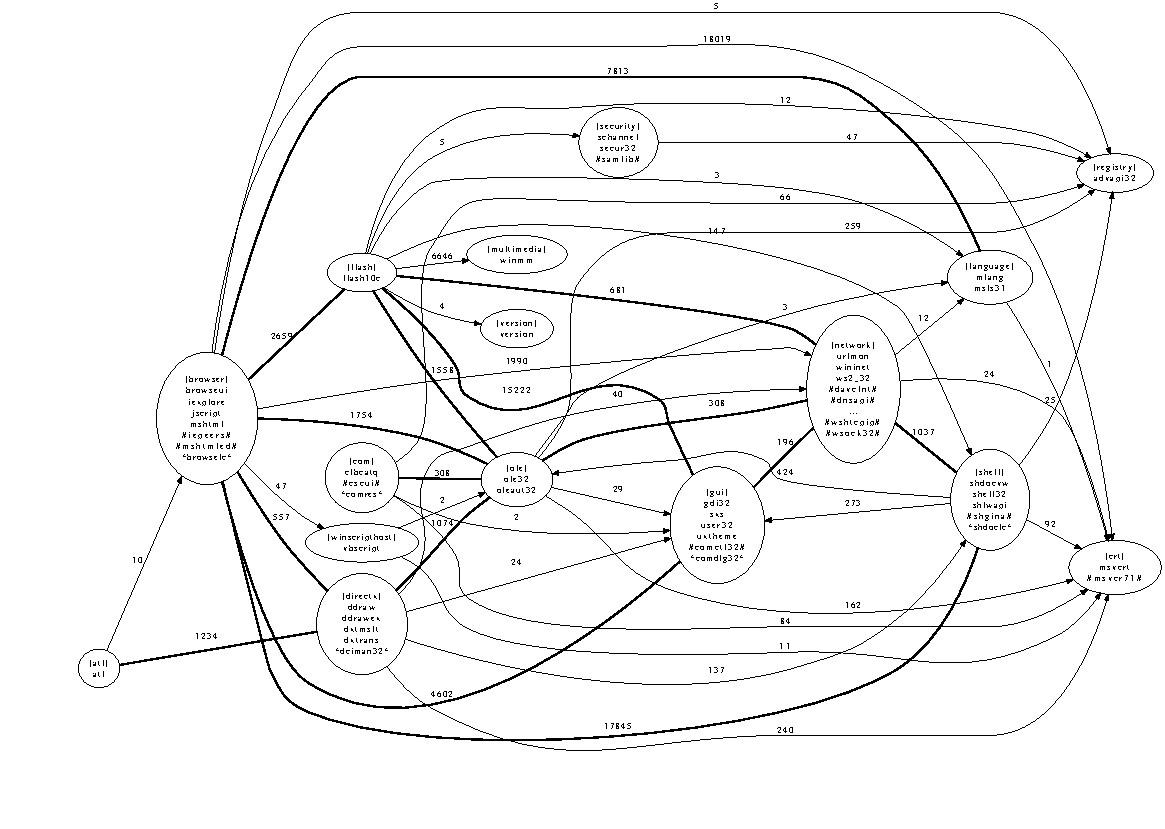
\includegraphics[keepaspectratio,width=0.8\textwidth,height=0.8\textheight]{depvis/ie-yt-proj.pdf}
\caption{Projection of the DLL dependency graph of Internet Explorer on Flash}
\label{fig:ie-proj}
\end{sidewaysfigure}

To further investigate the interactions resulting from the Flash module,
we project the visualization on {\tt flash10c.ocx} which is
the Flash ActiveX control.
Figure~\ref{fig:ie-proj} shows the projected graph.
We can see that Flash is interacting with the browser and multimedia modules.
The DLLs marked with {\bf \#x\#} neither use {\tt flash10c.ocx}
nor are they used by {\tt flash10c.ocx}.
In the {\tt network} group,
we can see that {\tt wsock32} is marked by {\bf \#x\#} but
{\tt ws2\_32} is not.
Windows has many network modules as shown in the {\tt network} group.
{\tt Wsock32} is an
older version of the winsock modules whereas {\tt ws2\_32} is the newer version.
This means the Flash player only uses the latest version of winsock rather
than the older version which is closer to the Unix socket API.
However, the older version is still used by some other modules
because otherwise {\tt wsock32} would have been labelled as {\bf *x*}.
The EXE dependency graph of the three browsers also shows that
both winsock modules are loaded by all three browsers.
The difference with projection is that projection is
more precise and shows the interaction between
the Flash module with the particular network module.
